\documentclass[11pt]{article}
\usepackage[margin=3cm]{geometry}
\geometry{letterpaper}                   
\usepackage{url}
\usepackage[colorlinks]{hyperref}
\hypersetup{
    citecolor = blue,
}
\usepackage{graphicx}
\usepackage{lipsum}
\usepackage{amssymb}
\usepackage{epstopdf}
\usepackage{algpseudocode}
\usepackage{amssymb, amsmath}
\usepackage[round]{natbib} 
\usepackage{parskip}
\DeclareGraphicsRule{.tif}{png}{.png}{`convert #1 `dirname #1`/`basename #1 .tif`.png}

%\title{Title}
%\author{Name 1, Name 2}
%\date{date} 
\setlength\parindent{0pt}

\renewcommand{\sectionautorefname}{\S}
\renewcommand{\subsectionautorefname}{\S}
\renewcommand{\subsubsectionautorefname}{\S}

\begin{document}

\thispagestyle{empty}

\begin{center}

\includegraphics[width=5cm]{ETHlogo.eps}

\bigskip


\bigskip


\bigskip


\LARGE{ 	Lecture with Computer Exercises:\\ }
\LARGE{ Modelling and Simulating Social Systems\\}

\bigskip

\bigskip

\small{Project Report}\\

\vspace{2cm}



\hline
\vspace{0.7cm}
\textbf{\LARGE{Opinion formation in networks of acquaintances}}\\
\vspace{1.1cm}
\hline

\bigskip

\bigskip

\bigskip

\LARGE{Romain Buchs \& Nicolas Habisreutinger}



\vspace{6cm}

Zurich\\
December 2018\\

\end{center}



\newpage

%%%%%%%%%%%%%%%%%%%%%%%%%%%%%%%%%%%%%%%%%%%%%%%%%

\newpage
\pagenumbering{roman}
\section*{Agreement for free-download}
\bigskip


\bigskip


\large We hereby agree to make our source code for this project freely available for download from the web pages of COSS. Furthermore, we assure that all source code is written by ourselves and is not violating any copyright restrictions.

\begin{center}

\bigskip


\bigskip


\begin{tabular}{@{}p{3.3cm}@{}p{6cm}@{}@{}p{6cm}@{}}
\begin{minipage}{3cm}

\end{minipage}
&
\begin{minipage}{6cm}
\vspace{2mm} \large Romain Buchs

 \vspace{\baselineskip}

\end{minipage}
&
\begin{minipage}{6cm}

\large Nicolas Habisreutinger

\end{minipage}
\end{tabular}


\end{center}
\newpage

%%%%%%%%%%%%%%%%%%%%%%%%%%%%%%%%%%%%%%%



% IMPORTANT
% you MUST include the ETH declaration of originality here; it is available for download on the course website or at http://www.ethz.ch/faculty/exams/plagiarism/index_EN; it can be printed as pdf and should be filled out in handwriting


%%%%%%%%%% Table of content %%%%%%%%%%%%%%%%%

\tableofcontents

\newpage

%%%%%%%%%%%%%%%%%%%%%%%%%%%%%%%%%%%%%%%

\pagenumbering{arabic}
\begin{center}
 \section*{Abstract}
 \parbox{0.9\linewidth}{\textit{Emergent phenomena such as the formation of opinion has long been studied in social sciences. It is only about twenty years ago, with the advent of modern computing, that simulating such systems became possible. The link between social system behaviour and statistical physics was only explored latter. This work is concerned with the dynamics of opinion formation which embodies one of the core question in the study of networks, specifically, whether the dynamics controls the structure of a network or whether the structure controls the dynamics. In 2006, Holme and Newman proposed a model that combines with a single parameter those two dynamics of opinion formation. They showed that their model undergoes a phase transition from a regime in which opinions are diverse to one in which most individuals are like-minded when applied to random graphs. In this work, we use their model to recover this phase transition on random graphs and apply it to scale-free graphs. We show that they exhibit the same critical exponents.}}
\end{center}¨.


\section{Introduction and Motivations}

A network is a set of entities, called nodes, which are inter-connected by links named edges \citep{Newman2003}. This kind of structure naturally occurs but is also the product of the human mind. Example of the former abound in biology or in materials. Example of the latter are the world-wide web, online social networks or financial networks \citep{Social_Network_book}. The study of those structures is formalized using graphs and is one of the pillars of discrete mathematics. Investigating the creation, the evolution, and the destruction of these structures in a wide variety of applications has led to a large body of knowledge \citep{Opinion_dynamics, Acemoglu2011}.

In the last decades, the rise of new numerical analytic tools has revolutionized research in social sciences and has helped to combine expertise in networks with complex real applications \citep{Social_Network_book}. Driven by these new possibilities, recent years have seen the shift of the research focus from small graphs to the statistical properties of large-scale networks \citep{Application, EcoloAppli}. An example of this trend is the study of opinion dynamics, which evolved from a purely sociology subject to more physical models \citep{Holme2002, Proskurnikov2016, Parsegov2017}. This new focus on physical model of opinion formation is sometimes criticized for its relative lack of connection to the `real world' societal interactions and behaviour \citep{Sobkowicz2009}. The study of the formation and evolution of opinions embodies a broader question of network dynamics: does dynamics controls the structure of the network or does the structure controls the dynamics?

It has been been observed that social interactions tend to lead towards a consensus or a polarization of the opinions \citep{Consensus, Proskurnikov2016}. Groups or communities are often composed of like-minded individuals. Societies segregates in groups that share common opinions or beliefs \citep{DiPrete2011}. But how do we end-up here? Do people form acquaintances with like-minded individuals or is their opinion influenced by their acquaintances? The former situation can be described using opinion formation models, such as the voter model \citep{Castellano, Sood2005}, whereas the latter can be described with models that use the ``homophily" principle \citep{homophily, homophily_Kiesner}. Those two radical models offer only a partial picture of human interactions. Real opinion formation dynamics must be governed by a mixture of those two phenomena: the network changing in response to opinion and opinion changing in response to the network. \citet{Holme2006} proposed probably the simplest model combining assortative network formation and opinion dynamics using a single parameter. Their model exhibits a phase transition between regimes in which one process or the other dominates the dynamics. In this work we investigate on this model and extend its application to scale-free graphs.

In \autoref{desc_model}, we describe in details the model proposed by \citet{Holme2006} and its expected behaviour. In \autoref{implementation}, we describe the implementation of the model in \texttt{python} used in this work. We then apply the model on random graphs and scale-free graphs in \autoref{sim_results}. We study the phase transition properties and discuss the differences between a random graph and a scale-free graph \citep{Fan2002_Scale-Free_graph}, which is a better representation of a real social network. We conclude in \autoref{conclusion}.

\section{Description of the Model}
\label{desc_model}
We want to reproduce the results presented in the Holme and Newman paper ``Non-equilibrium phase transition in the co-evolution of networks and opinions" published in 2006 (hereafter HN paper) and investigate on the transition phase presented in this paper. We describe below the model of opinion formation formulated by \cite{Holme2006}.

The network of acquaintances is composed of $N$ nodes, representing individuals and $M$ edges, representing the relations between people. Each node has an opinion $g_i$, where $i\in\{1, ..., G\}$, and $G$ is the total number of opinions in the network. It can change through time as some opinions can disappear in the dynamic evolution of the network \citep{Fu2008}. The behavior of networks with a small number of opinion is well known and has been intensively studied; especially with voter models \citep{Castellano, Sood2005, FernandezGracia2014}. However, there are numerous situations in which $G$ can be large. Example of this are religious beliefs \citep{Religious_Belief} and general opinion evolution in online social relationships \citep{Goh2006}.

In the following, we focus on arbitrarily large $G$ and assume that this number is proportional to the number of individuals present in the networks. This ratio is expressed as $\gamma =  \frac{N}{G} $. Edges and opinions are distributed randomly, creating a random network of people with relationships and with an individual opinion $g_i$. 

The simple model of opinion formation proposed by Holme and Newman has a discrete dynamics dictated by the parameter $\phi$. At each iteration: with probability $\phi$,  an edge is moved to lie between two like-minded individuals; and with probability $1-\phi$: an individual changes her opinion to agree with one of her acquaintances. The first possibility consists in a high social mobility. An individual will stop her relationship with whom she disagrees and begin a new one with a like-minded individual. The second possibility consists in a low social mobility. The individual prefers to change her opinion instead of creating new relations.

An iteration of the model can be summarized as follows (see \autoref{fig:model}). Pick randomly a node $i$. If the degree of the node is zero (i.e. $k_i=0$), do nothing. Otherwise: 
\begin{enumerate}
    \item With probability $\phi$: Pick randomly an edge attached to node $i$ and move the other end to a randomly picked node with opinion $g_i$ .
     \item With probability $1-\phi$: Pick $j$, a random neighbour of node $i$. Change the opinion of node $i$, $g_i$, to the one of node $j$, $g_j$.
\end{enumerate}
\begin{figure}
\centering
\begin{minipage}{.5\textwidth}
  \centering
  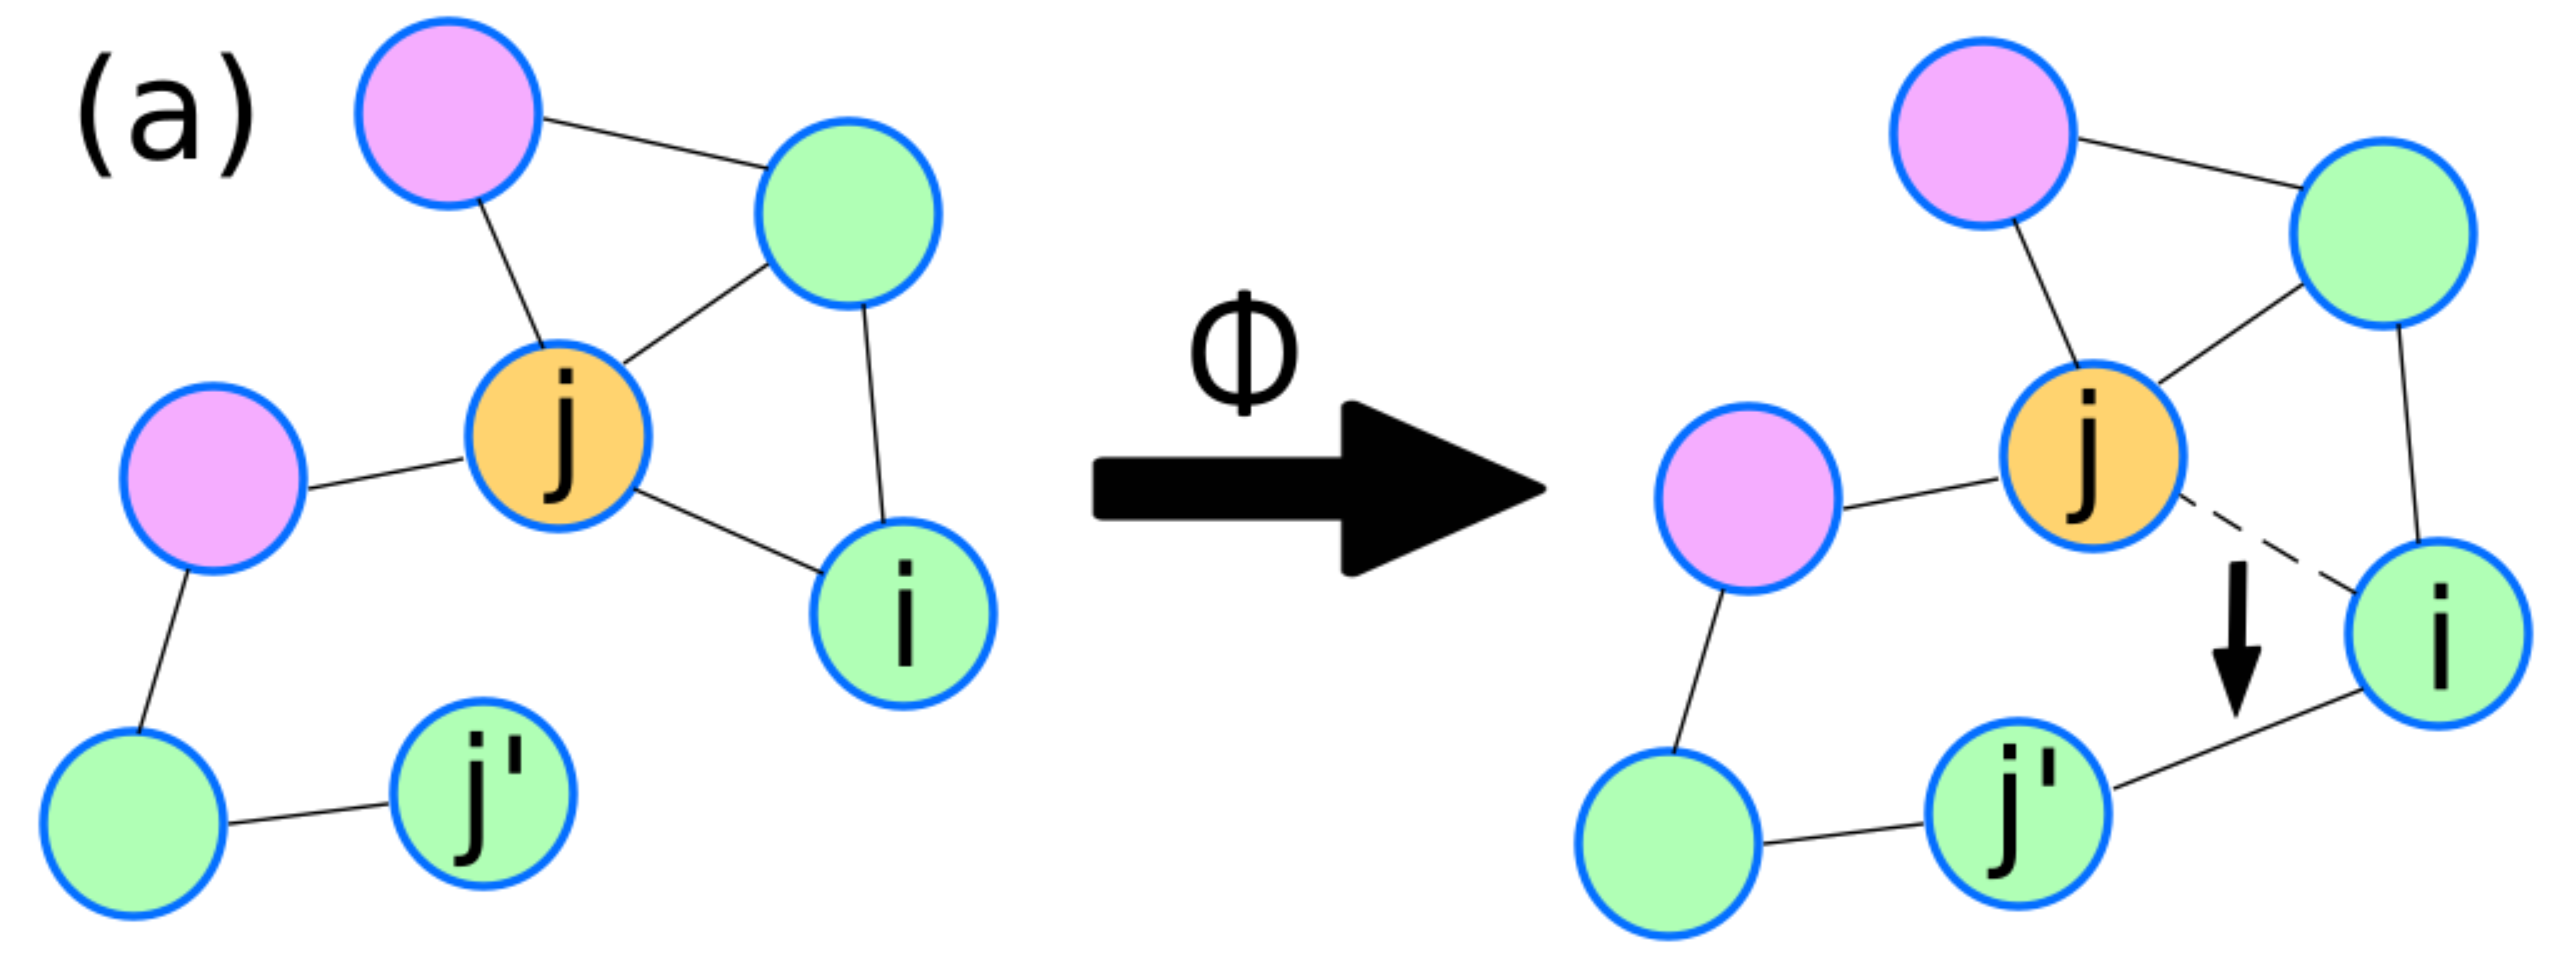
\includegraphics[width=0.9\linewidth]{figures/phi.png}
\end{minipage}%
\begin{minipage}{.5\textwidth}
  \centering
  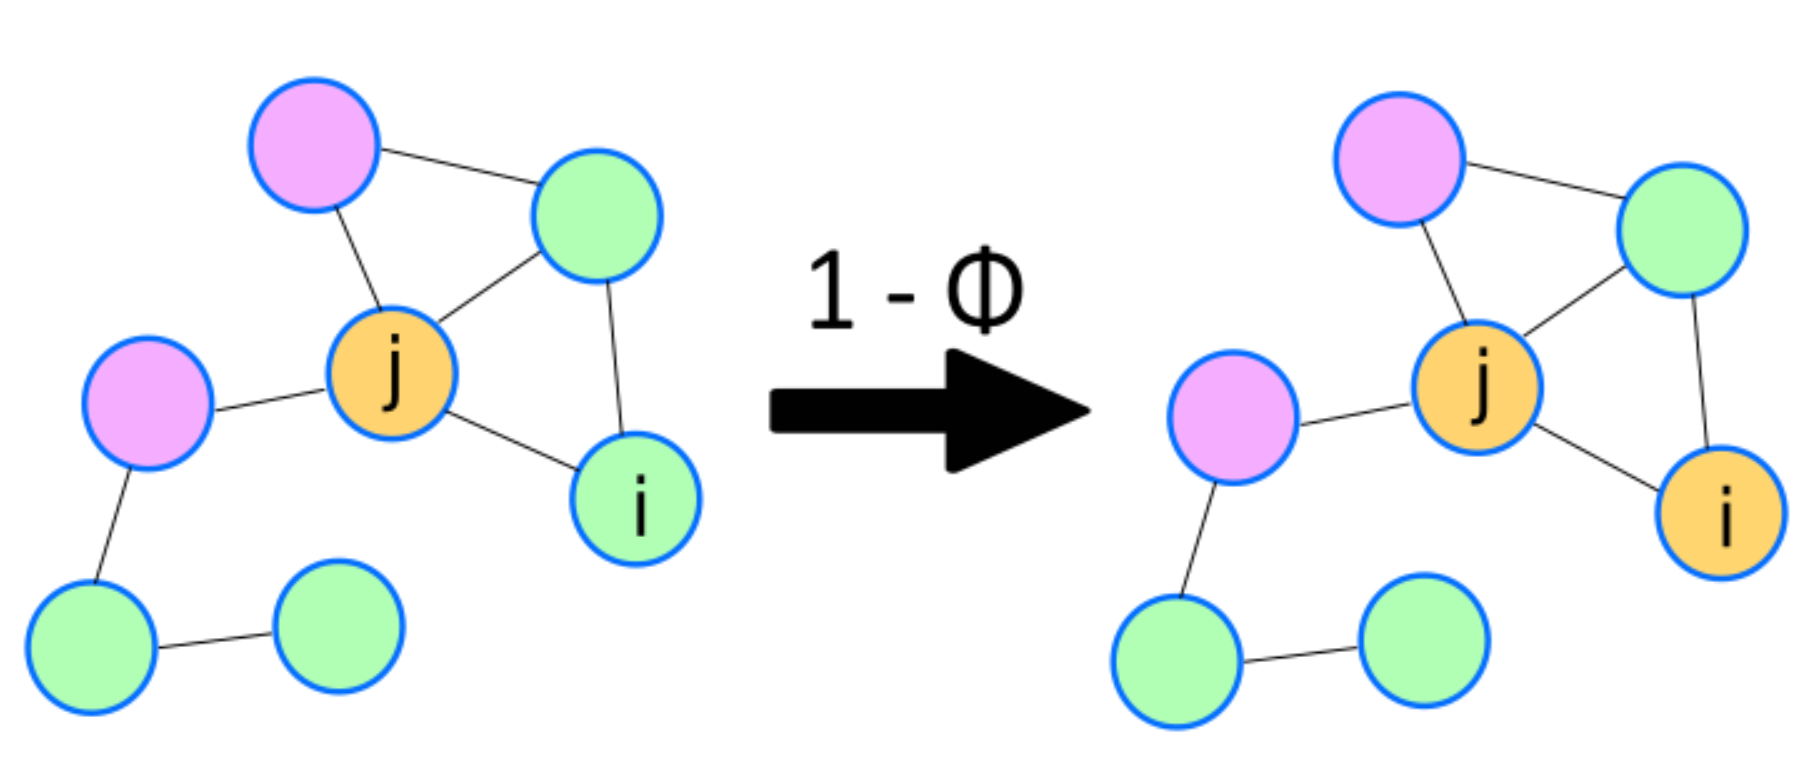
\includegraphics[width=0.9\linewidth]{figures/1-phi.png}
\end{minipage}
\caption{Illustration of the Holme-Newman model of opinion formation \citep{Holme2006}. Edges represent acquaintances between individuals and colors represent opinions. At each step, a node $i$ is randomly picked. In panel (a), with probability $\phi$,  a random neighbour $j$ is selected. The edge between $i$ and $j$ is deleted to the profit of the creation of a new relation between $i$ and $j'$, a randomly picked node with the same opinion as node $i$. In panel (b),  with probability $1 - \phi$, a random neighbour $j$ is selected and transmits its opinion to node $i$.}
    \label{fig:model}
\end{figure}

The total number of possible opinions $G$ and the number of edges $M$ being fixed, in the limit of large system size, the model has three parameters:
\begin{itemize}
    \item the average degree $\overline{k}$ = $\frac{2M}{N}$,
    \item the mean number of people holding an opinion $\gamma$ = $\frac{N}{G}$, and
    \item the probability $\phi$.
\end{itemize}
\subsection{Qualitative behavior of the model}
\label{sec:qul_behaviour}
The two possible updates of the algorithm decrease the number of nearest-neighbor node pairs with different opinions. We thus expect that ultimately the network will be divided into a set of separate components with all of their members holding the same opinion, respectively. The model converges to the so-called \textit{consensus state} where there is only homogeneous communities, i.e. there is no individual that has any acquaintance with whom they disagree.

Once the consensus state is reached, any update of the algorithm (i.e. any new iteration) randomly rearranges the edges within components.

We are interested in the number and sizes of the communities that are formed when reaching consensus. We consider the distribution $P(s)$ of the sizes $s$ of the communities at the consensus state (hereafter consensus communities). $P(s)$ is simply a normalized histogram of the community sizes. We assess the behaviour of $P(s)$ when taking extreme values of $\phi$:
\begin{itemize}
    \item $\phi\rightarrow 1$: Only the first step is allowed, i.e. only edges are moved between nodes and no opinion is modified. The edges are moved until all individuals holding the same opinion are in the same community with no acquaintance to someone holding a different opinion. The consensus communities are the sets of individuals holding the same opinion.  
    \item $\phi\rightarrow 0$: Only the second step is allowed, i.e. only opinions are changed and no edge is moved. The consensus communities consist of the initial components of the graph. Predicting the opinion of the components is more difficult. The `winning' one will depend on the order in which individuals are picked by the algorithm. In the regime $\Bar{k}>1$, there is a giant component in the random graph. At the consensus state, there is thus one large community and a distribution of small communities.
\end{itemize}
We see that by varying $\phi$ from 0 to 1, we move from a consensus state made of one giant community and a set of small ones to a consensus state made of small communities with constant average size $\gamma$. This is the behaviour of a system undergoing a continuous phase transition. We thus expect that this model has a phase transition when decreasing $\phi$. There is a critical value, $\phi_c$, at which a giant community of like-minded individuals forms. This implies that ``there is a transition between a regime in which the population holds a broad variety of views and one in which most people believe the same thing".  


\section{Implementation}
\label{implementation}
The model presented in \autoref{desc_model} is implemented in \texttt{python} using the \texttt{networkx} package\footnote{\url{https://networkx.github.io}}. The package offers the following features that are useful for this work: classes for graph objects, generators to create standard graphs and some basic drawing tools. We develop our own \texttt{OpinionGraph} class to embed our model\footnote{The code is available at \url{https://github.com/rbuchs/opinion-formation/tree/master/code.}}. An \texttt{OpinionGraph} object has the following attributes:
\begin{itemize}
    \item \texttt{OpinionGraph.simple\_graph} (boolean): a simple graph can have only single edges between nodes and no edge with itself, whereas a multi-graph can have parallel edges between two nodes and self-loops. We primarily work with multi-graphs, following the implementation described in the HN paper.     
    \item \texttt{OpinionGraph.internal\_graph} (\texttt{networkx.Graph} or \texttt{networkx.MultiGraph} depending on the value of \texttt{OpinionGraph.simple\_graph}): graph of the network we are studying. 
    \item \texttt{OpinionGraph.node\_with\_opinion} (list): the element $i$ of the list consist of all nodes with opinion $g_i$. 
    \item \texttt{OpinionGraph.conL} (list): the element $i$ of the list is the local consensus around node $i$, i.e. the number of acquaintances of node $i$ which have a different opinion. This allows to quickly check if the consensus is reached (by checking if the sum of the element in the list is zero).
\end{itemize}
When creating an instance of \texttt{OpinionGraph} the number of possible opinions, $G$, is required. Opinions are then randomly assigned to nodes of the internal graph as an attribute. A series of functions can create different types of initial \texttt{OpinionGraph}\footnote{\texttt{CreatePowerlawCluster}, \texttt{CreateNewmanWattsStrogatz}, \texttt{CreateBarbasiAlbert} and \texttt{CreateRandom}.}. To reproduce the result of the HN paper we use \texttt{CreateRandom} which creates a $G_{n,m}$ random graph with $n$ nodes and $m$ edges.

A number of functions of the class \texttt{OpinionGraph} directly acts on an instance of the class. \texttt{OpinionGraph.plot()} directly plots the instance and \texttt{OpinionGraph.summary()} produces a summary of the graph properties of interest for the model. 

The core of the model lies in the two possible steps outlined in \autoref{desc_model}. Those are implemented as \texttt{OpinionGraph.Step1()} and \texttt{OpinionGraph.Step2()}. Given a node $i$, those functions perform the step by directly acting on the \texttt{OpinionGraph}. For details of the implementation of the two steps we recommend looking directly at the code.

The algorithm in itself is implemented in the \texttt{OpinionAlgorithm.py} file. The function \texttt{OpinionAlgorithm.OneIteration()} performs one iteration of the model. It takes as inputs an \texttt{OpinionGraph}, the node on which the iteration is performed and a boolean that tells which step must be performed. The function then calls either \texttt{OpinionGraph.Step1()} or \texttt{OpinionGraph.Step2()}. To perform a finite number of iterations of the algorithm, the function \texttt{OpinionAlgorithm.simulation()} can be used. The function used to produce the results presented in this report is \texttt{OpinionAlgorithm. SimulationEndConsensus()} which performs iterations of the algorithm until the consensus is reached.

\section{Simulation Results and Discussion}
\label{sim_results}
In this section, we follow the HN paper structure. We try to reproduce the qualitative results presented in the paper. We then extend the discussion to scale-free graphs.

\subsection{Results of the Holme and Newman paper}
Reproducing the result of the HN paper requires running simulation of the model on large graphs (more than 1600 nodes) and with a large number of realizations ($10^4$). This is a challenge as a huge number of iterations are needed to reach the consensus state. The number of steps depend on the value of the parameter $\phi$; values of $\phi$ just bellow its critical value takes the longer. Although, we spent time trying to optimize the code, the result is somehow deceiving.  For example, reproducing exactly Figure 2 of the HN paper is out of reach in a decent amount of time with our implementation. After struggling a lot to obtain those results, we decided to restrain ourselves to smaller graphs and number of realizations. 

\subsubsection{Distribution of community sizes}
We are interested in the impact of the parameter $\phi$ on the distribution of community sizes $s$ at the consensus state. In \autoref{fig:Fig2_n800_m1600}, we show the normalized distribution of community sizes for three different values of $\phi$. We use networks with $n=800$, $\Bar{k}=4$ and $\gamma=10$. For each value of $s$ the number of communities is averaged over $10^3$ realizations. This can be compared to Figure 2 of the HN paper (hereafter HN-Fig 2). In their paper, they claim to ``bin logarithmically" the data which we do not fully understand. Indeed, looking closely at the data points of HN-fig 2, it appears that the values for $s\in\{1, 2, 3, 4, 5, 6\}$ are right above the ticks which do not indicate any binning. However, the next two data points lie between integer values which would indicate some sort of binning. Furthermore, for large values of $s$, the small number of data points indicates some sort of binning. This is a strange way of proceeding as it does not make much sense to talk about $s$ taking non-integer values. As we could not recover the exact binning of HN-Fig 2, we did not bin our data in \autoref{fig:Fig2_n800_m1600}. Our plot is qualitatively very similar to HN-Fig 2 apart from low values of $s$ for $\phi=0.96$ for which we have a higher probability compared to HN-Fig 2. This might be linked to the way the initial random graph is created or to the binning but we are not convinced by any of these explanations.
\begin{figure}[h]
    \centering
    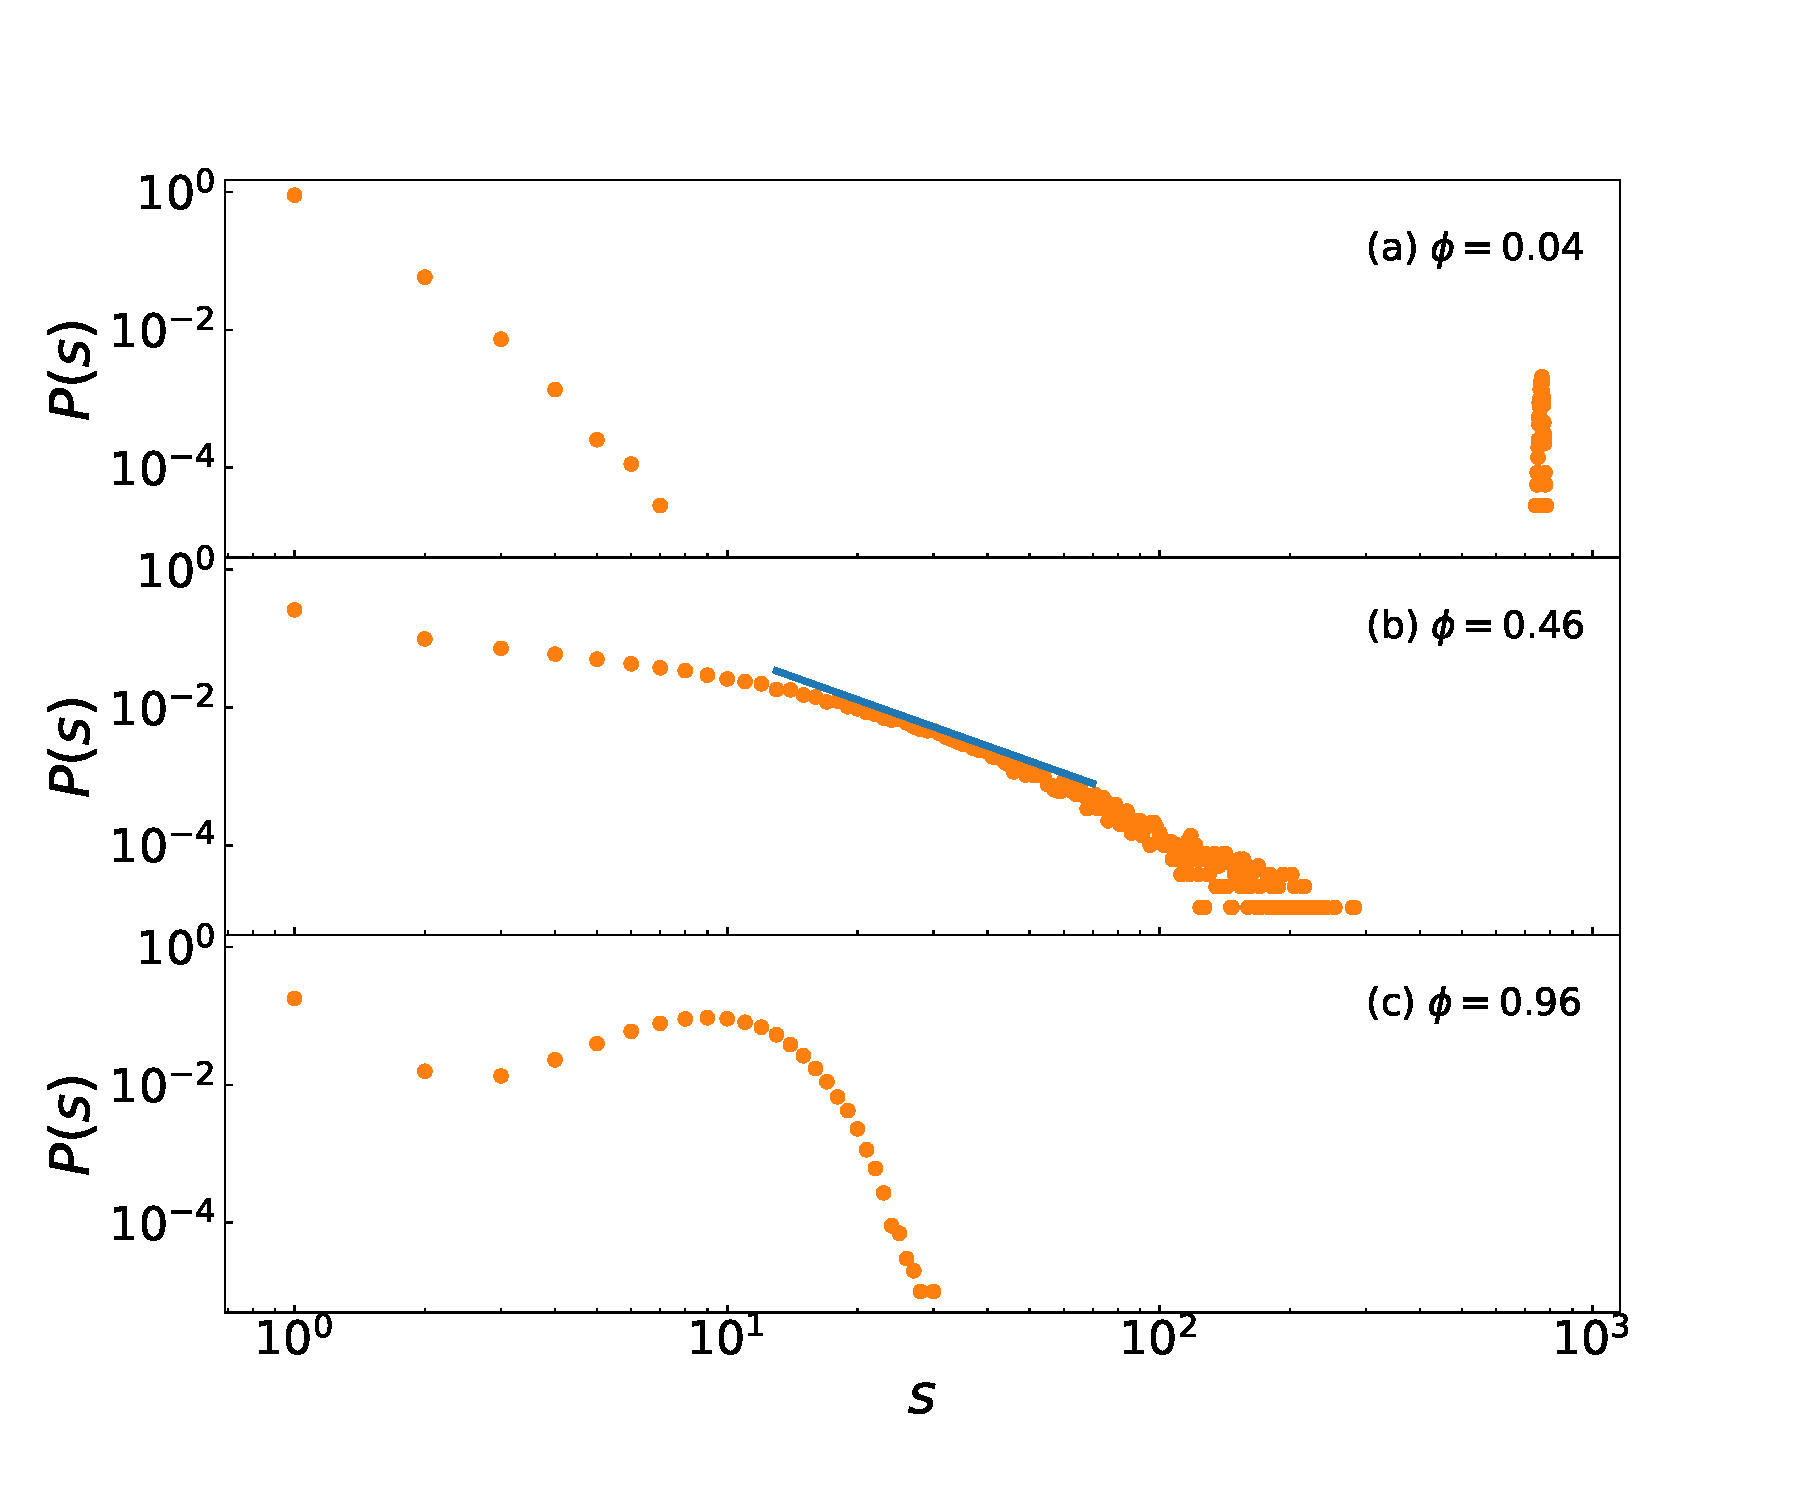
\includegraphics[width=0.7\linewidth]{figures/Fig2_n800_m1600.pdf}
    \caption{Normalized histograms of community sizes in the consensus state for three values of $\phi$ for graphs with $N = 800$, $M = 1600$ and $\gamma=10$. In panel (a), we have one giant community whereas in panel (c) there is no giant community and distribution of smaller ones. In panel (b), near the critical $\phi$, the distribution appears to follow a power law for part of its range. The blue line is a power-law fit in the range $s\in[15, 100]$ with exponent $\alpha\approx2.63$. The constant term of the fit is slightly increased to shift the line upwards on the plot for better visualization. Numerical data are averaged over $10^3$ realizations for each value of $s$ and $\phi$.}
    \label{fig:Fig2_n800_m1600}
\end{figure}

The qualitative behaviour described in \autoref{sec:qul_behaviour} is indeed present in \autoref{fig:Fig2_n800_m1600}. There is a transition between a regime with no giant community (for $\phi=0.96$, $P(s\gtrapprox40)=0$) to one with a giant community (for $\phi=0.04$, $P(s\gtrapprox600)>0$). At an intermediate value of $\phi=0.46$, the distribution of community sizes appears to follow a power law $P(s)\sim s^{-\alpha}$ over some range of sizes. This is a typical signature of criticality.  We measure the exponent $\alpha$ by running a regression using the data points in the range $s\in[15, 100]$. We find $\alpha\approx2.63$ which is inconsistent with the value presented in the HN paper ($\alpha=3.5 \pm 0.3$). This being said, the comparison with their result is difficult for a number of reasons. We do not know what is the range of the fit, especially if it is performed on the binned data and if they used all the realizations or if the fit is performed on their average. To account for the arbitrary range of the fit, we take all possible ranges of length 20 in between $s=15$ and $s=100$, i.e. all $[s_1, s_2+20]$, where $s_1\geq15$ and $s_2\leq80$. We then average the coefficient of those fits to find $\alpha=2.85 \pm 0.57$.

\subsubsection{Finite size scaling}
\label{sec:finite_size_scaling}
We want to perform a finite size scaling to better understand the transition between the two regimes of the model. The order parameter used for the model is chosen to be the size of the biggest community in the consensus state as a fraction of the system size, i.e.
\begin{equation}
    S = \max_s s\cdot N^{-1}.
\end{equation}
The arguments presented in \autoref{sec:qul_behaviour} and evidence from \autoref{fig:Fig2_n800_m1600} indicates that $S$ should be of size $O(N^{-1})$ for values of $\phi$ above the phase transition and $O(1)$ below it. Following the HN paper, we assume a scaling relation of the form 
\begin{equation}
\label{scaling}
S = N^{-a}F\left(N^b(\phi-\phi_c)\right)
\end{equation}
where $\phi_c$ is the critical value of $\phi$, $F$ is a universal scaling function and $a$ and $b$ are critical exponents.

We can use the property of universality of $F$ in \autoref{scaling} to estimate the critical $\phi$ and the exponents $a$ and $b$. We plot $N^aS$ as a function of $\phi$ in \autoref{fig:fig_HN_3}. This is similar to Figure 3 of the HN paper. The goal is to tune the value of $a$ such that the simulations with different number of individuals $N$ (but same $\Bar{k}$ and $\Bar{\gamma}$) cross in a single point: the critical point. Doing this precisely requires a high resolution (in $\phi$ and in number of realizations), which we do not have. We therefore directly use the value $a=0.61$ found by Holme and Newman and find it to be consistent with our data. In \autoref{fig:fig_HN_3}, this exponent results in the expected single point crossing. We estimate $\phi_c\approx0.465$, which is consistent with what Holme and Newman found ($\phi_c = 0.458 \pm 0.008$), but as can be seen from the one $\sigma$ shaded area, there is a lot of uncertainty on this measurement. 
\begin{figure}[h]
    \centering
    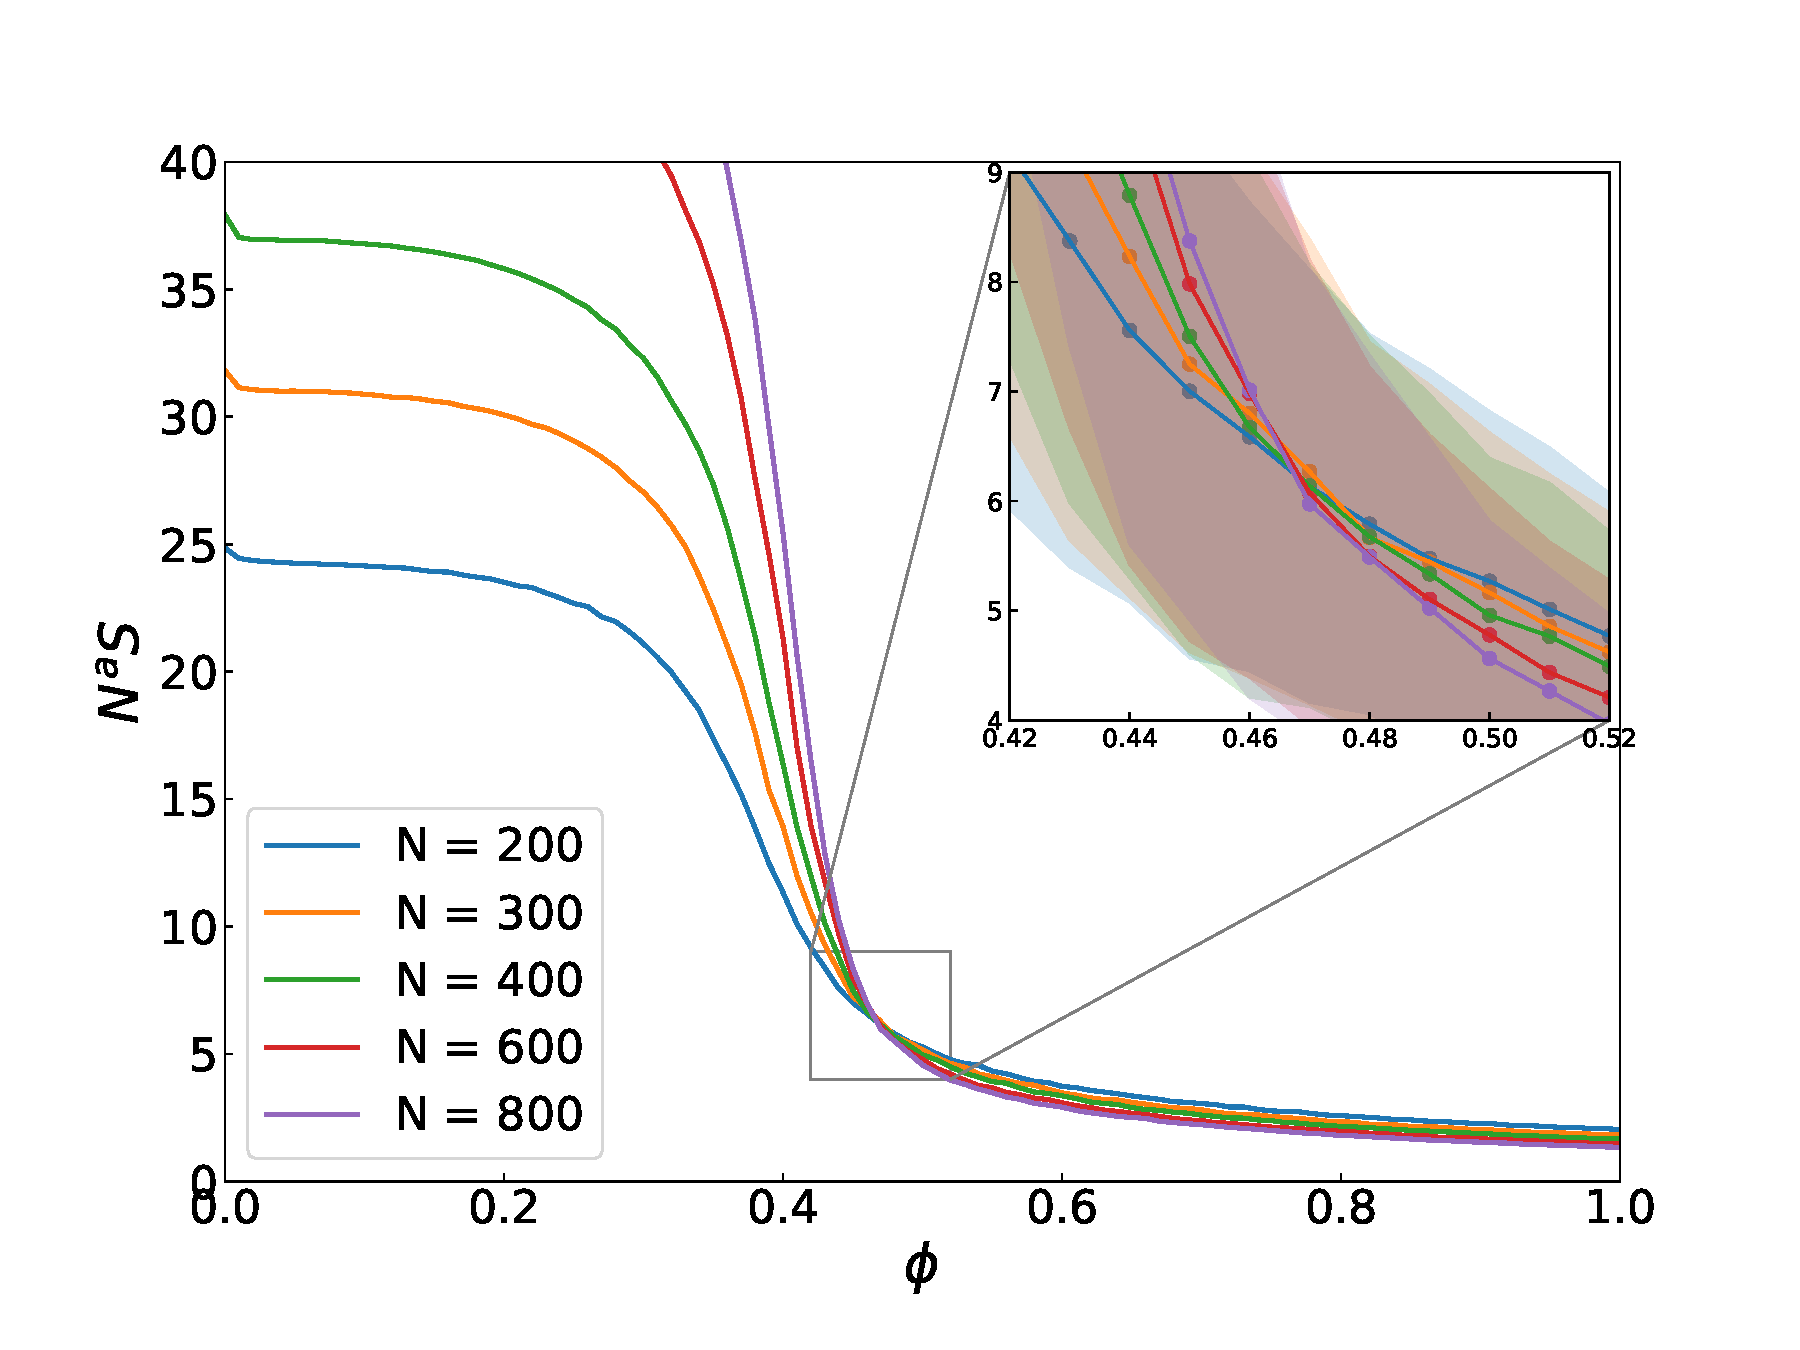
\includegraphics[width = 0.8\linewidth]{figures/Fig3_withInsert.pdf}
    \caption{Finite size scaling analysis for $\Bar{k}= 4$ and $\gamma = 10$. The coarse sampling in $\phi$ and the low number of realizations does not allow to estimate the critical point $\phi_c$ and the exponent $a$ precisely. The critical exponent $a=0.61$, taken from the HN paper, produces the single point crossing expected. We estimate $\phi_c \approx 0.465$, but as can be seen from the one $\sigma$ shaded area in the inset, the error is too large for a precise estimate. The size of the biggest community in the consensus state as a fraction of the system size $S$ is averaged over $10^3$ realizations.
}
    \label{fig:fig_HN_3}
\end{figure}

In \autoref{fig:fig_HN_3_errorbar}, we plot a single curve used in the finite size scaling with error bars. The uncertainty is rather small for $\phi\rightarrow0$ and $\phi\rightarrow1$. Close to the critical point, there is much more variability between realizations, which is a feature of criticality.
\begin{figure}[h]
    \centering
    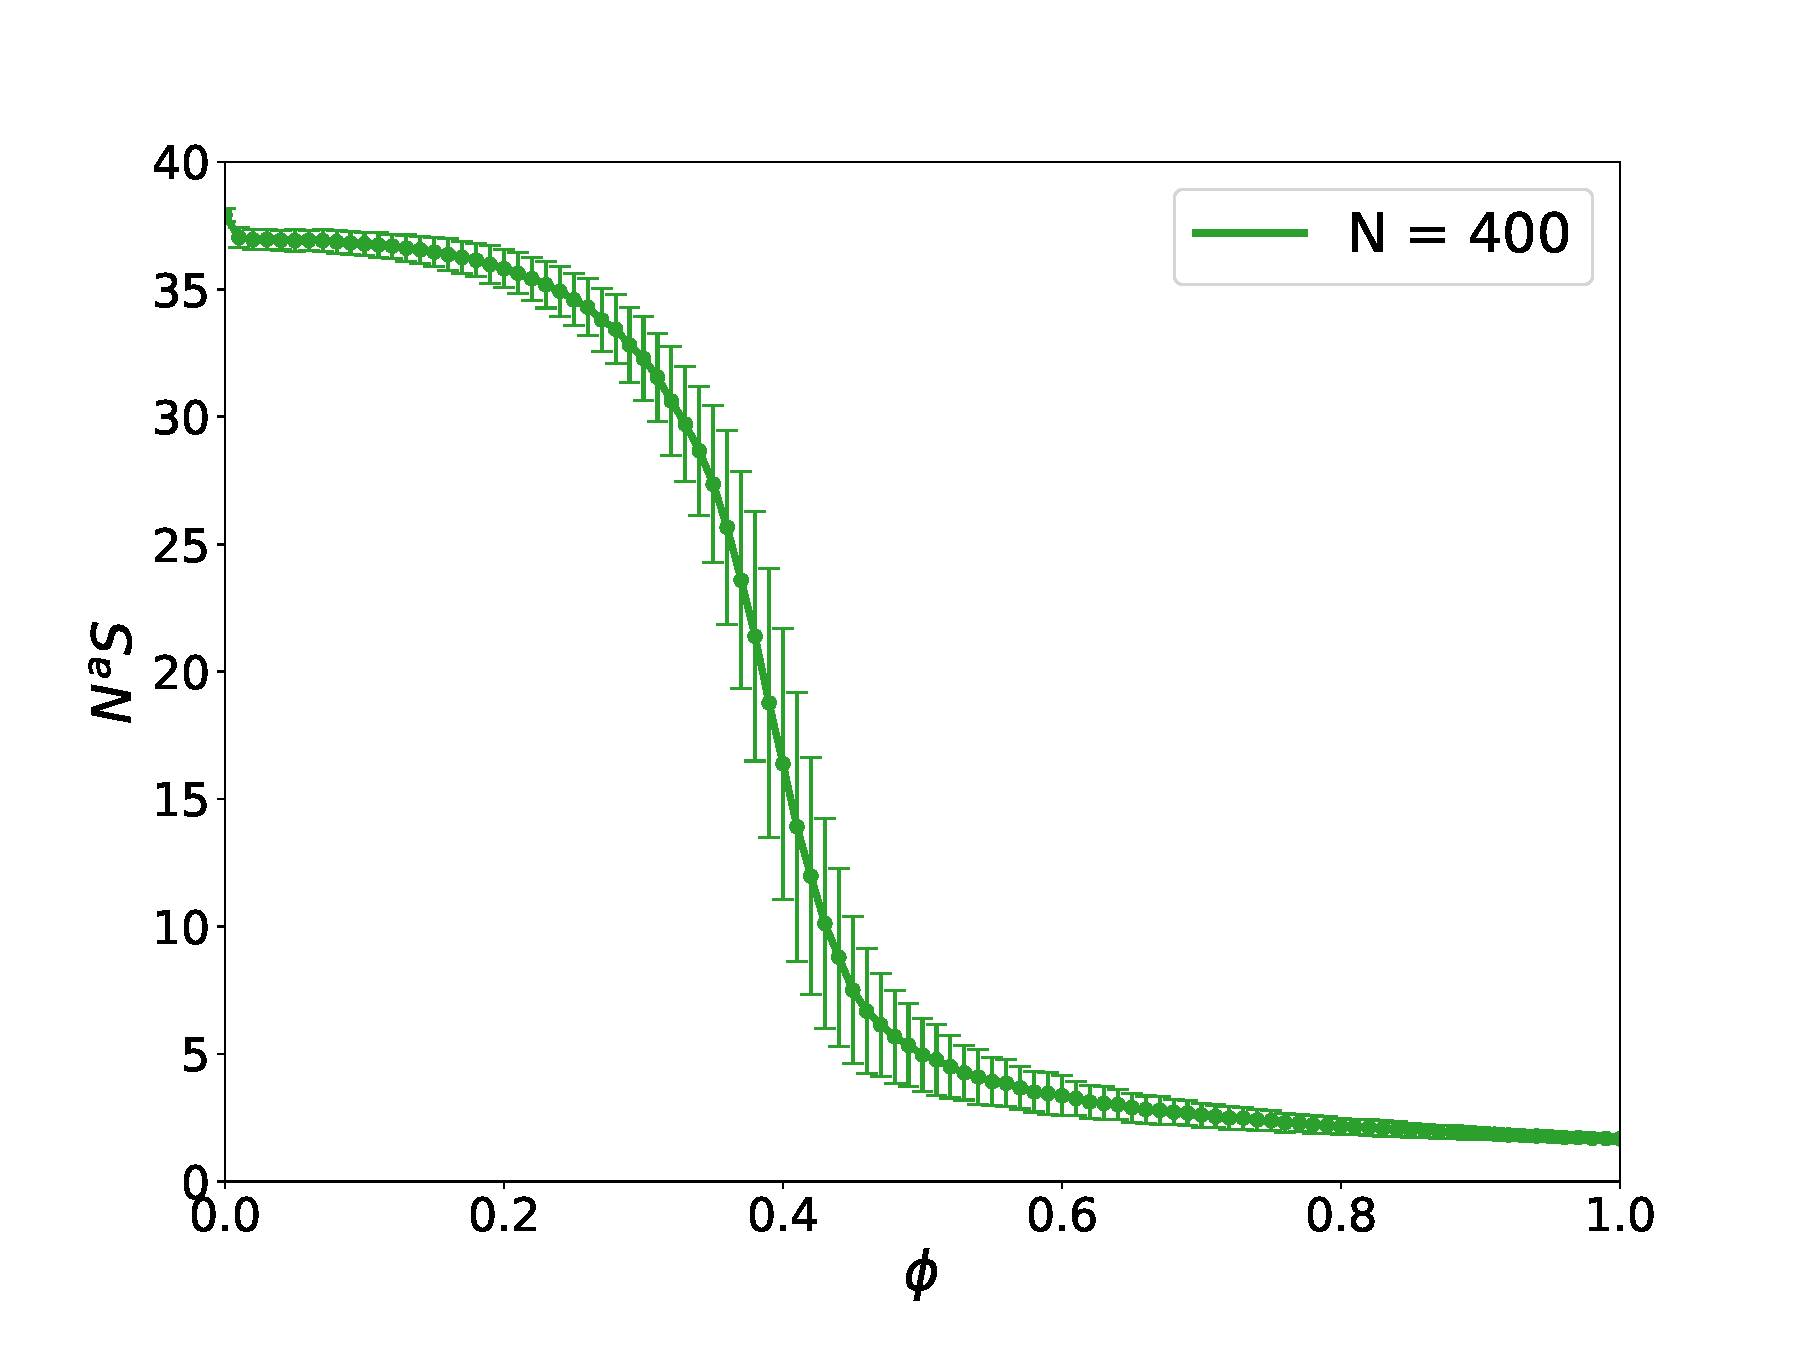
\includegraphics[width =0.8\linewidth]{figures/Fig3_n400_errorbar.pdf}
    \caption{The $N=400$ curve of the finite size scaling analysis for $\Bar{k}= 4$ and $\gamma = 10$ with one $\sigma$ error bars. Close to the critical point, there is much more uncertainty.
}
    \label{fig:fig_HN_3_errorbar}
\end{figure}

To obtain the value of the critical exponent $b$ we can use the value of $a$ previously found and plot $N^aS$ against $N^b(\phi-\phi_c)$. Again, the property of universality of $F$ means that the curves at different values of $N$ should collapse in the critical region for the correct value of $b$. Given the uncertainty we have on $\phi_c$, we do not try to estimate $b$ but instead check if the value found by Holme and Newman, $b=0.7$, leads to a data collapse in the critical region. In \autoref{fig:fig_HN_3_b}, we do this for two values of $\phi_c$: the one we estimated and the one presented in the Holme and Newman paper. Our value of $\phi_c$ leads to a better data collapse. This shows that the method is consistent.
\begin{figure}[h]
    \centering
    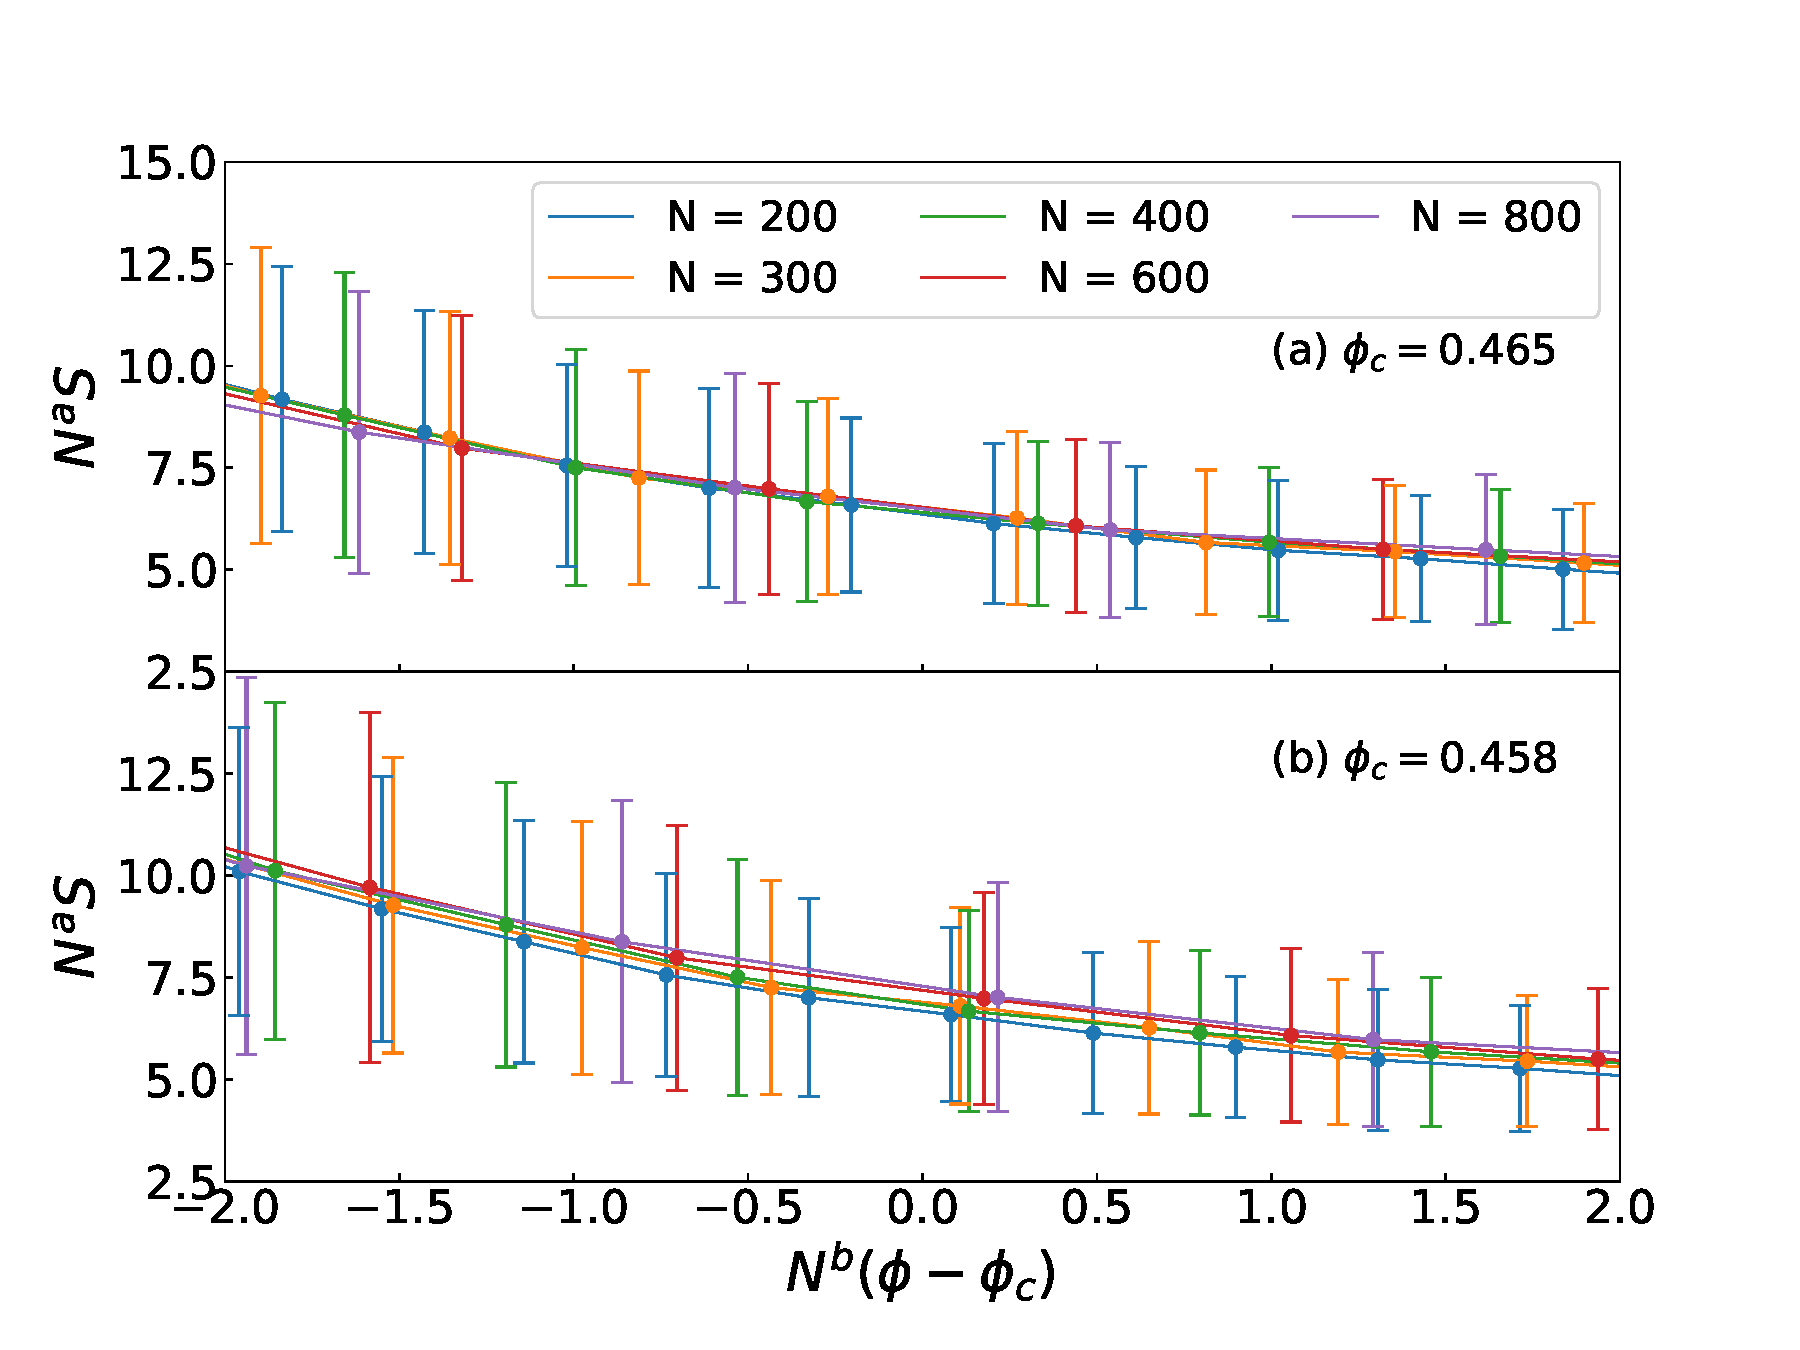
\includegraphics[width =0.8\linewidth]{figures/Fig3_n400_b.pdf}
    \caption{Scaling collapse with the exponent $b=0.7$ found by Holme and Newman for two values of $\phi_c$. In panel (a), the value of $\phi_c$ we estimated is used and in panel (b), the value estimated by Holme and Newman is used.}
    \label{fig:fig_HN_3_b}
\end{figure}

\subsection{Scale-free graph}
Some applications are not well described by random graphs. It has been shown that a wide variety of networks such as neural networks \citep{Watts1998}, networks of sexual relationships \citep{Liljeros2001}, collaborations between scientists \citep{Newman2001} or actors \citep{Watts1998, Barabasi1999}, or the world-wide web \citep{Albert1999} all share characteristics which are poorly modeled by random graphs. Indeed, those real world networks are highly clustered ``small worlds" with small average path length between nodes. Those networks have hubs which are highly connected nodes with a degree\footnote{The degree of a node is the number of connections it has with other nodes.} distribution often following a power law \citep{Barabasi1999}.

It has been shown that social networks (which are of primary interest in the case of opinion formation) do not have a random distribution of degrees (for example in the case of collaborations between scientists or actors). People are more likely to become friend with their friends' friends. Thus there is a higher probability of triangle relationships in the network. This can be described by scale-free graphs whose degree distribution follows a power law, i.e. $P(k) \sim k^{- \beta} $. The value of the parameter $\beta$ is generally observed to be between 2 and 3. Illustration of such a graph is presented in \autoref{fig:scale_free_illustration}.
\begin{figure}
    \centering
    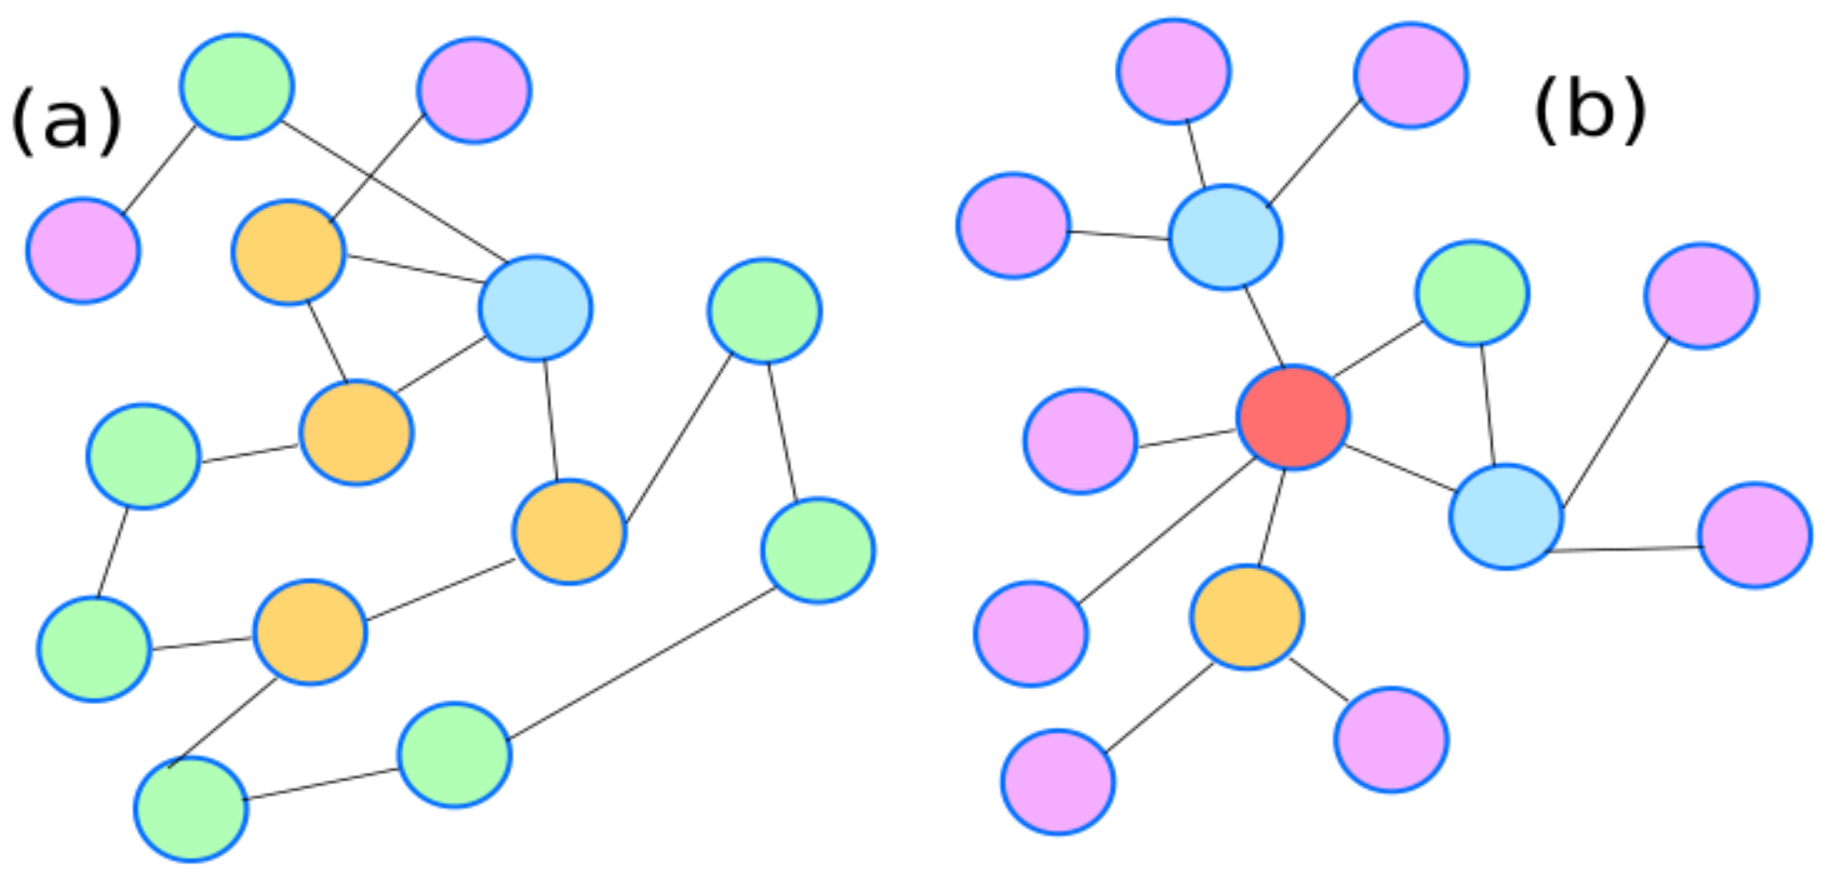
\includegraphics[width = 0.6\linewidth]{figures/Scalefree_graph.PNG}
    \caption{(a) Random graph. The degree distribution is random. (b) Scale-free graph. The degree distribution is power-law. The graph is organized around hubs which are highly connected to the rest of the nodes. Other nodes lie at the periphery of the graph and are only connected to a hub.}
    \label{fig:scale_free_illustration}
\end{figure}

To produce scale-free graphs, we use the \texttt{networkx} implementation of the Holme and Kim algorithm \citep{Holme2002}. It produces graphs with powerlaw degree distribution and approximate average clustering. The initial graph has three parameters: 
\begin{itemize}
    \item $N$ : the number of individuals,
    \item $m$ : the number of random acquaintances to add for each new individual, and
    \item $p$ : the probability of adding a triangle after adding a random acquaintance.
\end{itemize}
Initially all the individuals are part of a giant component which is more interlinked than a random graph. We thus expect a sharper transition between the two regimes.

We run the Holme and Newman model on a scale-free graph with parameters $m=3$, $p=0.2$ and $\gamma=10$, fixed. In \autoref{fig:Fig_scalefree}, we perform a finite size scaling similar to the one performed in \autoref{sec:finite_size_scaling}. We first notice that the transition from a regime with one big community to the one with a distribution of smaller communities is sharper.  We only run $10^2$ iterations with three values of $N$ which does not allow to precisely preform the finite size scaling. Using the same exponent $a=0.61$ as previously seems to give one crossing point. As the behaviour after the critical point diverges less between different value of $N$ than in a random graph, it is difficult to estimate $\phi_c\approx 0.69$. 

\begin{figure}
    \centering
    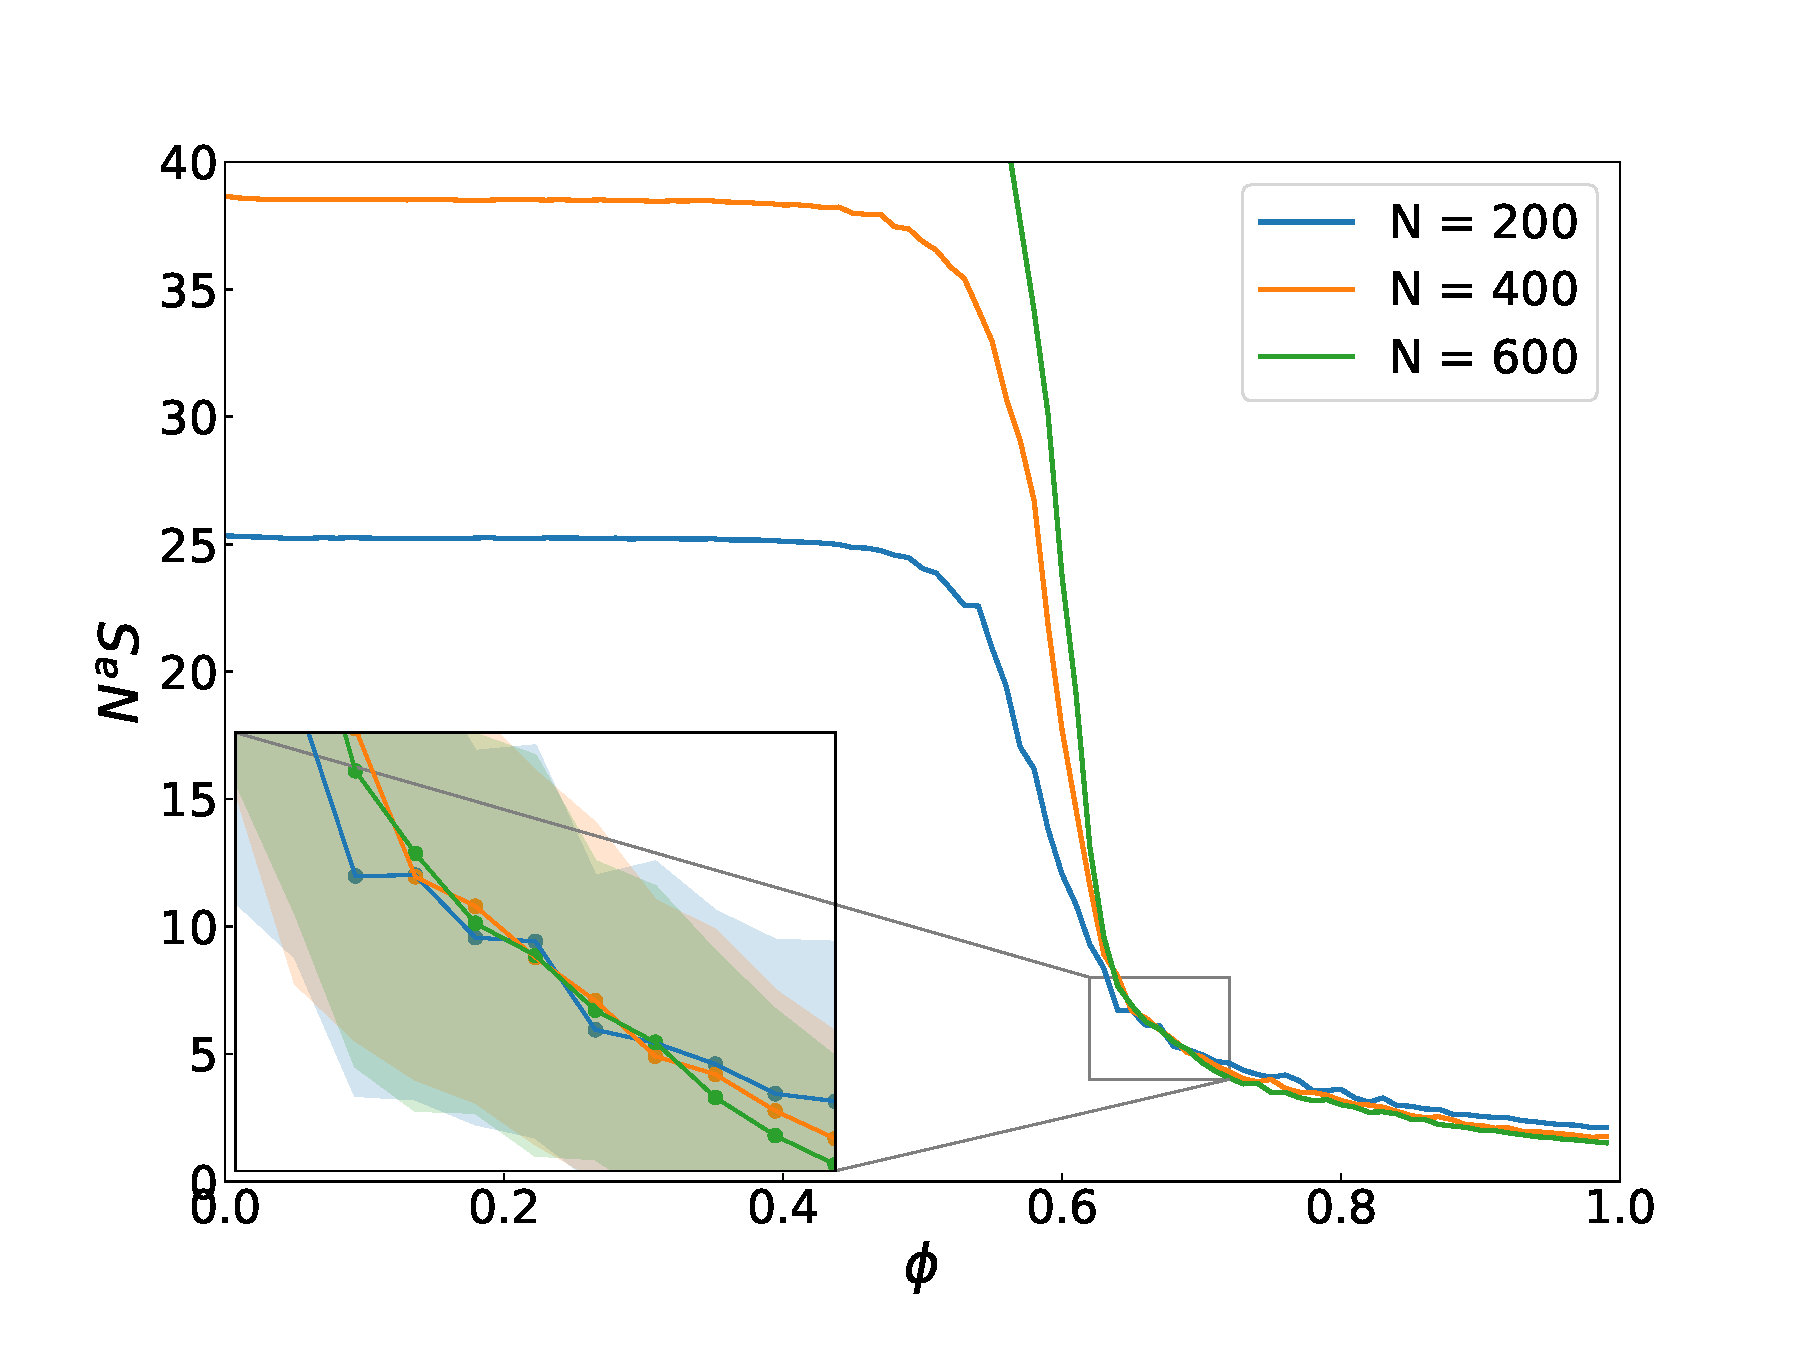
\includegraphics[width =\linewidth]{figures/Fig_scalefree.pdf}
    \caption{Finite size scaling analysis for a scale-free graph with $p=0.2$, $m=3$ and $\gamma=10$. The coarse sampling in $\phi$ and the low number of realizations does not allow to estimate the critical point $\phi_c$ and the exponent $a$ precisely. We find that using $a=0.61$ gives one crossing point.}
    \label{fig:Fig_scalefree}
\end{figure}

In \autoref{fig:fig_scale_free_b}, we plot $N^aS$ against $N^b(\phi-\phi_c)$ and use $b=0.7$ as previously. The expected data collapse occurs, leading us to conclude that $a=0.61$ and $b=0.7$ are indeed universal and are not affected by the type of graph. This result was expected as Holme and Newman showed that these exponents are universal on random graphs irrespective of the average degree $\Bar{k}$.

A scale-free graph with $m=3$ and $p=0.2$ has an average degree of $\bar{k}=2.40\pm0.04$ (computed on $10^4$ realizations). Compared to a random graph with a similar average degree the critical point is far higher, i.e. more of the first step are needed to reach a consensus in which a diversity of opinions are present. This means that preserving a diversity of opinions require a higher social mobility in a scale-free graph.

\begin{figure}
    \centering
    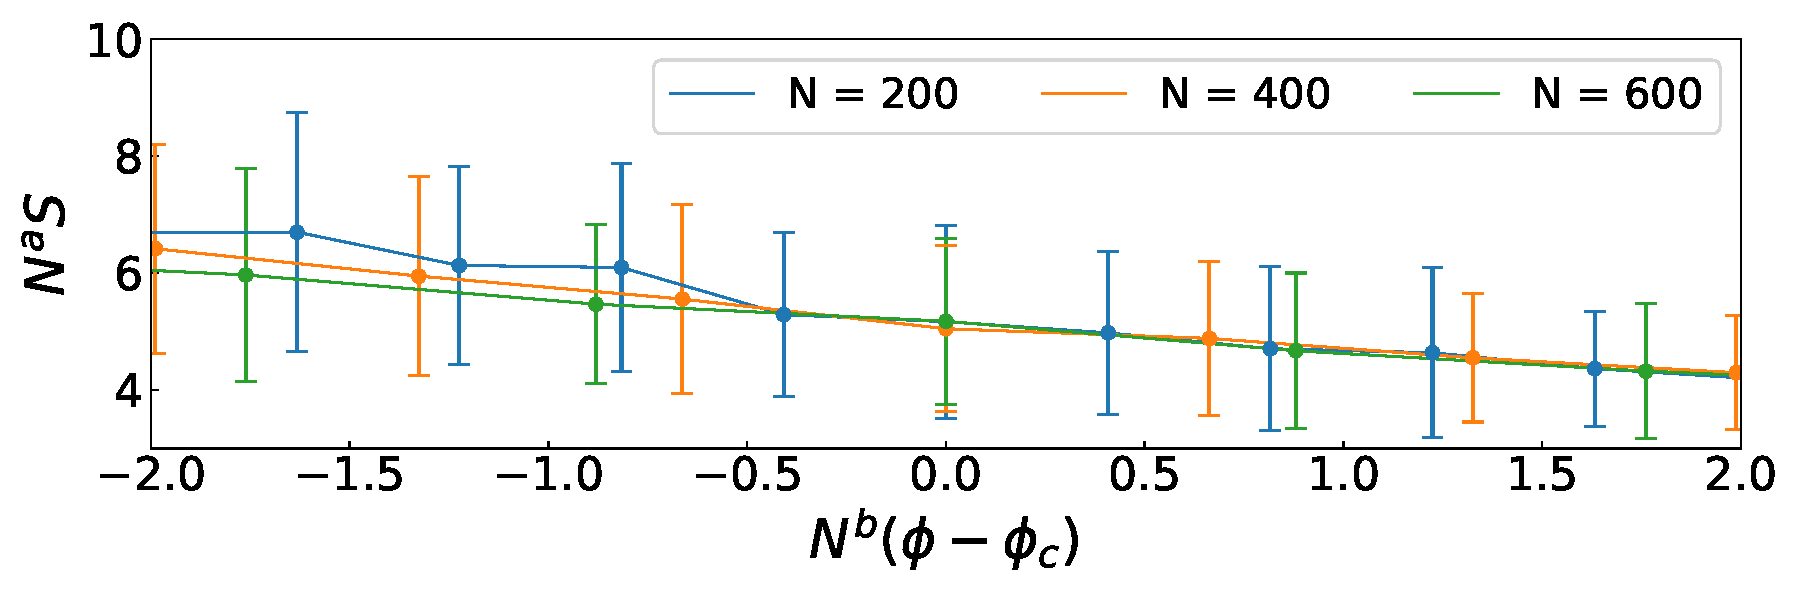
\includegraphics[width =\linewidth]{figures/Fig3_scalefree_b.pdf}
    \caption{Scaling collapse with the exponent $b=0.7$ found by Holme and Newman and $\phi_c=0.69$ for a scale-free graph with $p=0.2$ and $m=3$. The order parameter S is obtained by averaging $10^2$ realizations.}
    \label{fig:fig_scale_free_b}
\end{figure}

\section{Summary and Outlook} 
\label{conclusion}
In this work, we described the Holme-Newman model of opinion dynamics, probably the simplest model that combines the theory of homophily, where ``birds of a feather flock together" and the voter model, where opinions homogenize through the confrontation of peers, using a unique parameter $\phi$. By studying the size of the biggest community in the consensus state, we recovered the results found by Holme and Newman. The model exhibits a phase transition between a regime ($\phi\rightarrow0$) where a giant like-minded community exists and a regime ($\phi\rightarrow0$) where several middle-size like-minded groups exist. This phase transition is particularly interesting because it means that the resulting consensus state is very sensitive to the prominence of both models of opinion dynamics in the society. 

To study the dynamics of opinion formation, it is necessary to have a model representative of reality. One step towards this is the the use of scale-free graphs as initial networks. Indeed, we have seen that a feature of most human created networks is the power-law distribution of the degree of nodes. We have shown that using scale-free graphs produce the same phase transition (albeit with a sharper transition) with the exact same critical exponents.

The time constraints of this project coupled with the overtime spent in reproducing the results of \cite{Holme2006} did not allow us to fully explore its possibilities. Numerous refinement of it might be of interest. We list some of them below:
\begin{itemize}
    \item Individuals have a geographic localization. New links created between like-minded people should only happen between individuals which are close by. This is of interest only for real social networks and not for online social networks where this notion of distance is less relevant.
    \item Opinions are not discrete values. Everybody has different beliefs and opinions with small nuances. When the opinion of a node is changed for the one of its neighbour, the model could favour changes of opinion towards a similar one rather than a totally opposite one. We could also include a margin of tolerance for the consensus state. The consensus would stop being a set of homogeneous components and would be replaced with communities of similarly-minded people. 
    \item People are not uniform in their behaviour. In this model the nodes are identical apart from their individual opinion. We could include a parameter of `shyness' which could influence the tendency of each node to break a relationship but also to create new ones. We could also include the power of persuasion, i.e. the ability of an individual to convince another, and the stubbornness, i.e. the determination not to change one's opinion, into the model. This idea has been recently explored by \citet{Perez-Llanos2018}.
    \item Is $\phi$ a constant of time? A disruptive event, such as a terrorist attack, might affect the value of $\phi$ (i.e. the social mobility). It would be interesting to asses the effect of a radical change in the $\phi$-value during the simulation.
\end{itemize}

The models of opinion dynamics with a physics flavour, such as the one presented in this work, give an insight into the formation of consensus communities. Nonetheless, we need to be aware of the assumptions, as well as the limitations of the model. Modelling the behaviour of complex agents and their interactions with other agents is an arduous task. Keeping in mind that this is a simplified modelization of reality is necessary to avoid overstating the conclusions found by such models.

\bibliographystyle{apalike}
\bibliography{biblio}

\end{document}  



 
